% Latex template: mahmoud.s.fahmy@students.kasralainy.edu.eg
% For more details: https://www.sharelatex.com/learn/Beamer
\documentclass[11pt]{beamer}
\usetheme{Rochester}
\usecolortheme{dolphin}
\usepackage{amsmath,amssymb,amsthm}
\usepackage{mathtools}
\usepackage{graphicx}
\usepackage{tikz}
\usepackage{booktabs}
\usepackage{hyperref}
\usepackage{algorithm}
\usepackage{algpseudocode}
\setbeamertemplate{navigation symbols}{}% myadditions
\usepackage{makecell}

\usepackage{amsmath,amssymb,amsthm}
\usepackage{mathtools}

\usepackage{biblatex}
\usepackage{cleveref}
\usetikzlibrary{arrows.meta, shapes.multipart, positioning, calc}

\tikzset{
  treenode/.style={
    rectangle, draw=black, rounded corners, minimum width=16mm, minimum height=8mm,
    align=center, font=\footnotesize
  },
  term/.style={treenode, fill=gray!10},
  internal/.style={treenode, fill=blue!5},
  edge/.style={-Latex, line width=1pt},
  oplabel/.style={font=\small\bfseries}
}

\addbibresource{example.bib}

% myadditions

\usepackage{mathtools}
%\usepackage{cleveref}

\newcommand{\R}{\mathbb{R}}
\newcommand{\E}{\mathbb{E}}
\newcommand{\Prob}{\mathbb{P}}
\newcommand{\vecc}[1]{\boldsymbol{#1}}

\title[]{Conditional Copula models using loss-based Bayesian Additive Regression Trees (Ongoing)}% Presentation title

\author[]{\small{\underline{Tathagata Basu} \inst{1} \and F. Leisen \inst{2} \and C. Vila \inst{3} \and K. Wilson  \inst{1}}}								% Presentation author
\institute{\inst{1} Newcastle University, UK \\\inst{2} Kings College London, UK \\\inst{3} Duke Kunshan University, China}
\date{\scriptsize{14th Nov, 2025}}									% Today's date	

\begin{document}
	
	% Title page
	% This page includes the information defined earlier including title, author/s, affiliation/s and the date
	\begin{frame}
		\titlepage
	\end{frame}

    \AtBeginSection[]
{
    \begin{frame}
        \frametitle{Table of Contents}
        \tableofcontents[currentsection]
    \end{frame}
}

	\section{Motivation}

    \begin{frame}[allowframebreaks]{}
        \begin{figure}
	\centering
	\includegraphics[width = 0.95\linewidth]{"LE_hist.pdf"}
\end{figure}

\begin{figure}
	\centering
	\includegraphics[width = 0.95\linewidth]{"LE_scatter.pdf"}
\end{figure}

    \end{frame}
    
    \section{Conditional Copulas}

    \begin{frame}{Definition of a Copula}
    \begin{block}{Copula}
    A \emph{copula} is a $d$-dimensional distribution function $C:[0,1]^d\to[0,1]$ with uniform $\mathrm{Unif}(0,1)$ marginals such that
    \vspace{0.5em}
    \begin{itemize}
    \item For any continuous marginals $F_1,\dots,F_d$ and joint $H$ there exists a unique copula $C$ \footfullcite{sklar:1959} s.t.
    \[ H(y_1,\dots,y_d)=C\big(F_1(y_1),\dots,F_d(y_d)\mid \theta\big). \]
    \item Alternatively,
    \[ C\big(u_1,\dots,u_d\mid \theta\big) = H\left(F_1^{-1}(u_1),\dots,F_d^{-1}(u_d)\right). \]
    \end{itemize}
    \end{block}
    \end{frame}
    

    \begin{frame}{Conditional Copula: Motivation}
    \begin{itemize}
    \item A \emph{conditional copula} captures the dependence between $Y_1,\dots,Y_k$ given covariates or other variables.
    \item Two common perspectives:
    \begin{enumerate}
    \item Copula parameters vary with covariates: $C_{\theta(x)}(\cdot)$.
    \item Full conditional copula: copula of conditional marginal distributions, e.g.,
    \[ C_{x}(u_1,u_2)=\Prob\big(F_{1x}(y_1)\le u_1,\; F_{2x}(y_2)\le u_2 \big). \]
    \end{enumerate}
    \end{itemize}
    \end{frame}
    
    
    \begin{frame}{Conditional Sklar's Theorem}
    \begin{itemize}
        \item For continuous conditional marginals $F_{1x},\dots,F_{dx}$ and joint conditional cdf $H_{x}(\cdot|x)$,
    there exists a conditional copula $C_{x}$\footfullcite{patton2006} such that
    \[ H_{x}(y_1,\dots,y_d) = C_{x}\big( F_{1x}(y_1),\dots, F_{dx}(y_d) \mid \theta(x)\big). \]
    That is the copula may vary w.r.t.~$x$.
    \item Alternatively,
    \[ C\big( u_1,\dots, u_d \mid \theta(x)\big) = H_{x}(F^{-1}_{1x}(u_1),\dots,F^{-1}_{dx}(u_d)). \]
    \end{itemize}
    \end{frame}
    
    \section{Loss based BART}

    \begin{frame}{Single Regression Tree Model}
    Let $T$ denote a regression tree with internal nodes (decision rules) and terminal nodes with values 
    \[
    M = \{\mu_1, \mu_2, \dots, \mu_{n_L(T)}\},
    \]
    where $n_L(T)$ is the number of terminal nodes.
    
    
    Each observation is predicted via
    \[
    Z_i = g(x_i, T, M) + \epsilon_i,
    \]
    with noise
    \[
    \epsilon_i \sim \mathcal{N}(0, \sigma^2).
    \]
    Here, $g(\cdot)$ maps $x_i$ to its terminal-node value.
    \end{frame}
    
    \begin{frame}{Example Regression Tree}
    \centering
    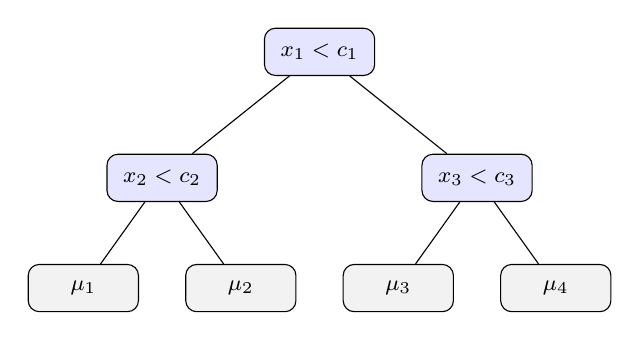
\begin{tikzpicture}[
    level 1/.style={level distance=16mm, sibling distance=40mm},
    level 2/.style={level distance=14mm, sibling distance=20mm},
    every node/.style={font=\footnotesize},
    treenode/.style={rectangle, draw=black, rounded corners, minimum width=14mm, minimum height=6mm, align=center},
    internal/.style={treenode, fill=blue!10},
    term/.style={treenode, fill=gray!10}
    ]
    
    
    % Root
    \node[internal] (root) {$x_1 < c_1$}
    child { node[internal] (n1) {$x_2 < c_2$}
    child { node[term] (l1) {$\mu_1$} }
    child { node[term] (l2) {$\mu_2$} }
    }
    child { node[internal] (n2) {$x_3 < c_3$}
    child { node[term] (l3) {$\mu_3$} }
    child { node[term] (l4) {$\mu_4$} }
    };
    
    
    \end{tikzpicture}
    \vspace{2em}

    \alert{$n_L(T) = 4$}
    \end{frame}
    
    \begin{frame}{Sum-of-Trees Model (BART)}
    We can extend regression tree model for $m$ trees \footfullcite{chipman_BART}.
    
    
    \[
    Z_i = \sum_{t=1}^m g(x_i, T_t, M_t) + \epsilon_i,
    \]
    with noise $\epsilon_i \sim \mathcal{N}(0, \sigma^2)$.
    
    
    Here:
    \begin{itemize}
    \item $T_t$ is the $t$-th tree,
    \item $M_t = \{\mu_1,\dots,\mu_{n_L(T_t)}\}$ its leaf values,
    \item $n_L(T_t)$ the number of terminal nodes.
    \end{itemize}
    \end{frame}

    \begin{frame}{Loss-Based Prior for Tree Topology}
    Serafini et al.\footfullcite{serafini2024lossbasedpriortreetopologies} proposed an objective prior by minimising the loss due to misspecification of a tree:
    \begin{itemize}
    \item \textbf{Information loss} $\equiv 0$
    \item \textbf{Complexity loss}
    \end{itemize}
    
    
    The loss in complexity is defined as:
    \[
    \omega\, n_L(T_t) - \zeta\, \Delta(T_t),
    \]
    where
    \begin{itemize}
    \item $\omega \ge 0$ and $\zeta \in \mathbb{R}$ are prior parameters,
    \item $n_L(T_t)$ is the number of terminal nodes of tree $T_t$,
    \item $\Delta(T_t)$ is the difference between right and left terminal nodes.
    \end{itemize}
    \end{frame}

    \begin{frame}{Loss in information}
    \centering
    
    \begin{minipage}{0.48\textwidth}
    \centering
    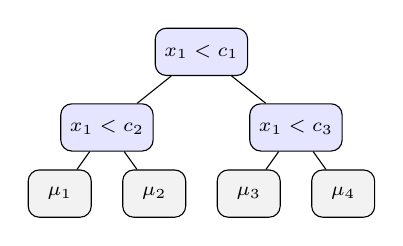
\begin{tikzpicture}[
    level 1/.style={level distance=16mm, sibling distance=40mm},
        level 2/.style={level distance=14mm, sibling distance=20mm},
        every node/.style={font=\footnotesize},
        treenode/.style={rectangle, draw=black, rounded corners, minimum width=8mm, minimum height=6mm, align=center, font=\scriptsize},
    internal/.style={treenode, fill=blue!10},
    term/.style={treenode, fill=gray!10},scale = 0.6
    ]
    \node[internal] (r) {$x_1 < c_1$}
    child { node[internal] {$x_1 < c_2$}
    child { node[term] {$\mu_1$} }
    child { node[term] {$\mu_2$} }
    }
    child { node[internal] {$x_1 < c_3$}
    child { node[term] {$\mu_3$} }
    child { node[term] {$\mu_4$} }
    };
    \end{tikzpicture}
    \end{minipage}
    \hfill
    \begin{minipage}{0.48\textwidth}
    \centering
    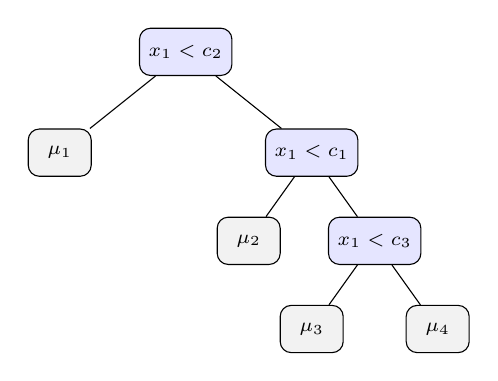
\begin{tikzpicture}[
    level 1/.style={level distance=16mm, sibling distance=40mm},
        level 2/.style={level distance=14mm, sibling distance=20mm},
        every node/.style={font=\footnotesize},
        treenode/.style={rectangle, draw=black, rounded corners, minimum width=8mm, minimum height=6mm, align=center, font=\scriptsize},
    internal/.style={treenode, fill=blue!10},
    term/.style={treenode, fill=gray!10},scale = 0.8
    ]
    \node[internal] (r2) {$x_1 < c_2$}
    child { node[term] {$\mu_1$}
    }
    child { node[internal] {$x_1 < c_1$}
    child { node[term] {$\mu_2$} }
    child { node[internal] {$x_1 < c_3$}
    child { node[term] {$\mu_3$} }
    child { node[term] {$\mu_4$} }
    }} % optional duplicate leaf to maintain four terminals
    ;
    \end{tikzpicture}
    \end{minipage}
        
    
    \end{frame}
    
    \begin{frame}{Hierarchical Prior Specification}
    This leads to the hierarchical prior:
    \begin{align}
    T_t, M_t &\sim \pi(T_t)\pi(M_t \mid T_t), \\
    \pi(T_t) &\propto \exp\left( \omega n_L(T_t) - \zeta \Delta(T_t) \right), \\
    \pi(M_t \mid T_t) &= \prod_{j=1}^{n_L(T_t)} \pi( \mu_j \mid T_t ).
    \end{align}
    where $\pi$ denotes a prior density.
    \end{frame}



    \section{Conditional Copula Modelling}

    \begin{frame}{Hierarchical Model for Conditional Copula}
    Let
    \[
    \theta(x_i) \coloneqq \alert{h}\left( \sum_{t=1}^m g(x_i, T_t, M_t) \right); \qquad 1 \le i \le n.
    \]
    
    
    Then
    
    \begin{align}\label{eq:bayes:hier}
    \begin{split}
    u_{1i}, u_{2i} \mid \theta(x_i) &\sim c\Big(u_{1i}, u_{2i} \mid \alert{h}\Big( \sum_{t=1}^m g(x_i, T_t, M_t) \Big)\Big),\\
    T_t &\propto \exp\Big(\omega n_L(T_t) - \zeta \Delta(T_t)\Big),\\
    \pi(M_t \mid T_t) &\propto \prod_{j=1}^{n_L(T_t)} \pi(\mu_j \mid T_t), \quad t=1,2,\dots,m.
    \end{split}
    \end{align}
    
    \end{frame}

    \begin{frame}[allowframebreaks]{Posterior Sampling}
    Let 
\begin{align*}
	&(T_{-k},M_{-k})\\
    &\coloneq \left\{(T_1,M_1),\cdots,(T_{k-1},M_{k-1}),(T_{k+1},M_{k+1}),\cdots(T_m,M_m)\right\},
\end{align*}
We want sample $(T_k, M_k)$ from 
\begin{equation*}
	(T_k,M_k)\mid T_{-k},M_{-k}, \sigma^2_{k}, U_1, U_2, X
\end{equation*}
Let $R_{ik} = \sum_{t\not=k}g(x_i, T_t, M_t)$ and $R_{\cdot k}\coloneqq(R_{1k},R_{2k},\cdots,R_{nk})$ such that
\begin{align}\label{eq:post:res}
	\begin{split}
		&\pi(T_k,M_k \mid R_{\cdot k}, \sigma^2_{k}, U_1,U_2, X) \\
        &\propto \pi(T_k)\prod_{i=1}^{n}c\left(u_{1i},u_{2i}\mid h\left(R_{ik}+g(x_i, T_k, M_k)\right)\right)\prod_{j=1}^{n_L(T_k)}\pi(\mu_j\mid T_k)
	\end{split}
\end{align}
\end{frame}

\begin{frame}[allowframebreaks]{RJ-MCMC Algorithm}

        We consider a proposal function to generate a new pair $\left(T_k^\ast, M_k^\ast\right)$ at the $(\eta+1)$-th iteration given by:
\begin{align}\label{eq:prop}
	q\left(T_k^\ast, M_k^\ast \mid T_k^{\eta},M_k^{\eta}\right) = q\left( T_k^\ast\mid T_k^{\eta}\right) q\left(M_k^\ast\mid T_k^\ast, T_k^{\eta}, M_k^{\eta}\right).
\end{align}
Here, $q\left( T_k^\ast\mid T_k^{\eta}\right)$ denotes the tree proposals given by:
\begin{itemize}
	\item \textsc{grow}: Randomly choose a terminal node and split it into two terminal nodes
	\item \textsc{prune}: Randomly choose a parent of terminal nodes and turn into a terminal node
	\item \textsc{change}: Randomly choose an internal node and assign a new splitting rule
	\item \textsc{swap}: Randomly choose a parent-child pair of internal node and swap their splitting rules
\end{itemize}
\newpage
For terminal node values, we use $q\left(M_k^\ast\mid T_k^\ast, T_k^{\eta}, M_k^{\eta}\right)$ given by:
\begin{itemize}
	\item For \textsc{grow} we consider the $j$-th leaf to be grown to $j_L$ and$j_R$ so,
	$q\left(M_k^\ast\mid T_k^\ast, T_k^{\eta}, M_k^{\eta}\right)$ = $\pi_{prop}(\mu_{j_L})\times\pi_{prop}(\mu_{j_R})$
	\item For \textsc{prune} we consider the $j_L$th and $j_R$th leaves to be pruned then $q\left(M_k^\ast\mid T_k^\ast, T_k^{\eta}, M_k^{\eta}\right)$ = $\pi_{prop}(\mu_j)$
\end{itemize}
where $\pi_{prop}$ denotes the proposal density function.
\newpage
We define the acceptance probability in the following way:
\begin{align*}
    &\alpha\left(T_k^{\eta},M_k^{\eta};T_k^\ast, M_k^\ast\right)\\
	&= \frac{\mathcal{L}(U_1,U_2\mid T_k^\ast,M_k^\ast)\pi(T_k^\ast,M_k^\ast)q\left(T_k^{\eta},M_k^{\eta}\mid T_k^\ast, M_k^\ast\right)}
	{\mathcal{L}(U_1,U_2\mid T_k^{\eta},M_k^{\eta})\pi(T_k^{\eta},M_k^{\eta}) q\left(T_k^\ast, M_k^\ast \mid T_k^{\eta},M_k^{\eta}\right)}.
\end{align*}
where 
\begin{equation*}
	\mathcal{L}(U_1,U_2\mid T_k, M_{k})\coloneqq \prod_{i=1}^{n}c\left(u_{1i},u_{2i}\mid h\left(R_{ik}+g(x_i, T_k, M_k)\right)\right).
\end{equation*}
    \end{frame}
    \begin{frame}{BART Move: \textsc{grow}}
    \centering

    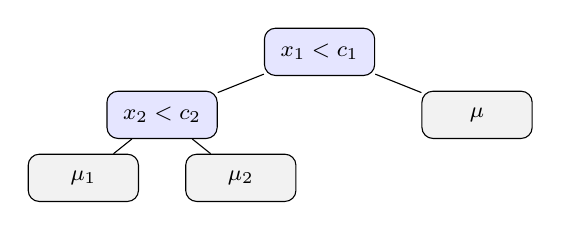
\begin{tikzpicture}[
    level 1/.style={level distance=8mm, sibling distance=40mm},
    level 2/.style={level distance=8mm, sibling distance=20mm},
    every node/.style={font=\footnotesize},
    treenode/.style={rectangle, draw=black, rounded corners, minimum width=14mm, minimum height=6mm, align=center},
    internal/.style={treenode, fill=blue!10},
    term/.style={treenode, fill=gray!10}
    ]
    
    
    % Root
    \node[internal] (root) {$x_1 < c_1$}
    child { node[internal] (n1) {$x_2 < c_2$}
    child { node[term] (l1) {$\mu_1$} }
    child { node[term] (l2) {$\mu_2$} }
    }
    child { node[term] (l3) {$\mu$}
    };
    
    
    \end{tikzpicture}

    \vspace{5mm}
    Grown version
    \vspace{5mm}

    
    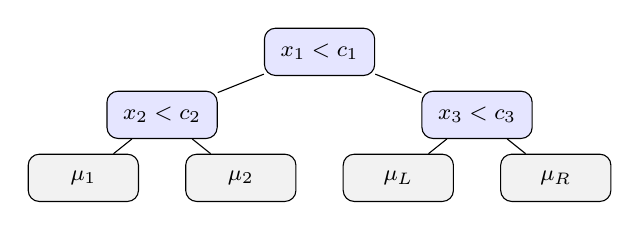
\begin{tikzpicture}[
    level 1/.style={level distance=8mm, sibling distance=40mm},
    level 2/.style={level distance=8mm, sibling distance=20mm},
    every node/.style={font=\footnotesize},
    treenode/.style={rectangle, draw=black, rounded corners, minimum width=14mm, minimum height=6mm, align=center},
    internal/.style={treenode, fill=blue!10},
    term/.style={treenode, fill=gray!10}
    ]
    
    
    % Root
    \node[internal] (root) {$x_1 < c_1$}
    child { node[internal] (n1) {$x_2 < c_2$}
    child { node[term] (l1) {$\mu_1$} }
    child { node[term] (l2) {$\mu_2$} }
    }
    child { node[internal] (n2) {$x_3 < c_3$}
    child { node[term] (l3) {$\mu_L$} }
    child { node[term] (l4) {$\mu_R$} }
    };
    
    
    \end{tikzpicture}
    \end{frame}
    
    
    \begin{frame}{BART Move: \textsc{prune}}
    \centering
    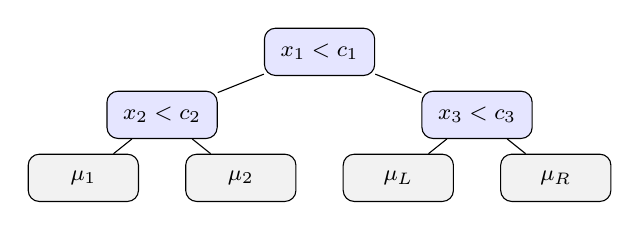
\begin{tikzpicture}[
    level 1/.style={level distance=8mm, sibling distance=40mm},
    level 2/.style={level distance=8mm, sibling distance=20mm},
    every node/.style={font=\footnotesize},
    treenode/.style={rectangle, draw=black, rounded corners, minimum width=14mm, minimum height=6mm, align=center},
    internal/.style={treenode, fill=blue!10},
    term/.style={treenode, fill=gray!10}
    ]
    
    
    % Root
    \node[internal] (root) {$x_1 < c_1$}
    child { node[internal] (n1) {$x_2 < c_2$}
    child { node[term] (l1) {$\mu_1$} }
    child { node[term] (l2) {$\mu_2$} }
    }
    child { node[internal] (n2) {$x_3 < c_3$}
    child { node[term] (l3) {$\mu_L$} }
    child { node[term] (l4) {$\mu_R$} }
    };
    
    
    \end{tikzpicture}

    \vspace{5mm}
    Pruned version:
    \vspace{5mm}
    

    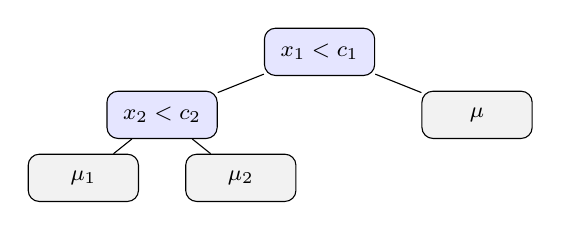
\begin{tikzpicture}[
    level 1/.style={level distance=8mm, sibling distance=40mm},
    level 2/.style={level distance=8mm, sibling distance=20mm},
    every node/.style={font=\footnotesize},
    treenode/.style={rectangle, draw=black, rounded corners, minimum width=14mm, minimum height=6mm, align=center},
    internal/.style={treenode, fill=blue!10},
    term/.style={treenode, fill=gray!10}
    ]
    
    
    % Root
    \node[internal] (root) {$x_1 < c_1$}
    child { node[internal] (n1) {$x_2 < c_2$}
    child { node[term] (l1) {$\mu_1$} }
    child { node[term] (l2) {$\mu_2$} }
    }
    child { node[term] (l3) {$\mu$}
    };
    
    
    \end{tikzpicture}
    
    \end{frame}
    
    
    \begin{frame}{BART Move: \textsc{swap}}
    \centering
    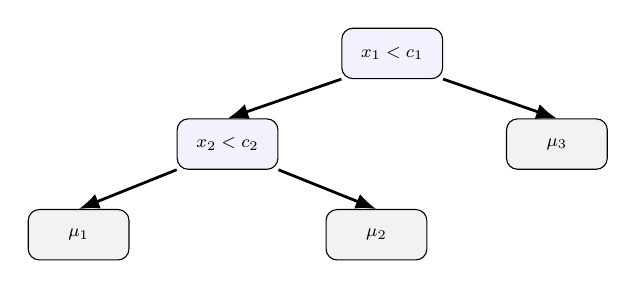
\begin{tikzpicture}[scale=0.8, every node/.style={scale=0.8}]
    \node[internal] (sP) {$x_1 < c_1$};
    \node[internal, below left=5mm and 8mm of sP] (sC) {$x_2 < c_2$};
    \node[term, below right=5mm and 8mm of sP] (sR) {$\mu_3$};
    \node[term, below left=5mm and 6mm of sC] (sCL) {$\mu_1$};
    \node[term, below right=5mm and 6mm of sC] (sCR) {$\mu_2$};
    \draw[edge] (sP.south west) -- (sC.north);
    \draw[edge] (sP.south east) -- (sR.north);
    \draw[edge] (sC.south west) -- (sCL.north);
    \draw[edge] (sC.south east) -- (sCR.north);
    \end{tikzpicture}
    
    
    \vspace{5mm}
    Swapped version:
    
    
    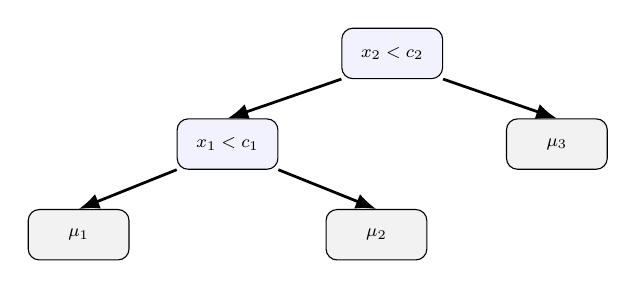
\begin{tikzpicture}[scale=0.8, every node/.style={scale=0.8}]
    \node[internal] (sP2) {$x_2 < c_2$};
    \node[internal, below left=5mm and 8mm of sP2] (sC2) {$x_1 < c_1$};
    \node[term, below right=5mm and 8mm of sP2] (sR2) {$\mu_3$};
    \node[term, below left=5mm and 6mm of sC2] (sCL2) {$\mu_1$};
    \node[term, below right=5mm and 6mm of sC2] (sCR2) {$\mu_2$};
    \draw[edge] (sP2.south west) -- (sC2.north);
    \draw[edge] (sP2.south east) -- (sR2.north);
    \draw[edge] (sC2.south west) -- (sCL2.north);
    \draw[edge] (sC2.south east) -- (sCR2.north);
    \end{tikzpicture}
    \end{frame}
    
    
    \begin{frame}{BART Move: \textsc{change}}
    \centering
    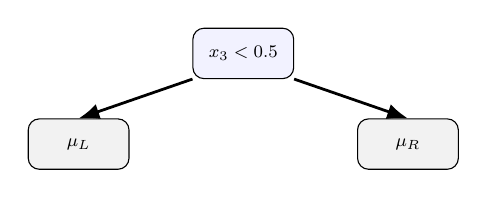
\begin{tikzpicture}[scale=0.8, every node/.style={scale=0.8}]
    \node[internal] (c1) {$x_3 < 0.5$};
    \node[term, below left=5mm and 8mm of c1] (cL) {$\mu_L$};
    \node[term, below right=5mm and 8mm of c1] (cR) {$\mu_R$};
    \draw[edge] (c1.south west) -- (cL.north);
    \draw[edge] (c1.south east) -- (cR.north);
    \end{tikzpicture}
    
    
    \vspace{4mm}
    After change:
    
    
    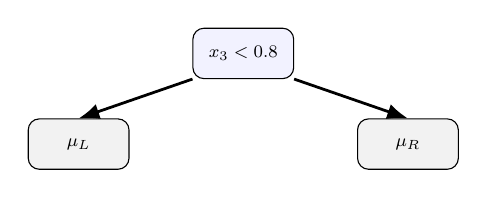
\begin{tikzpicture}[scale=0.8, every node/.style={scale=0.8}]
    \node[internal] (c2) {$x_3 < 0.8$};
    \node[term, below left=5mm and 8mm of c2] (c2L) {$\mu_L$};
    \node[term, below right=5mm and 8mm of c2] (c2R) {$\mu_R$};
    \draw[edge] (c2.south west) -- (c2L.north);
    \draw[edge] (c2.south east) -- (c2R.north);
    \end{tikzpicture}
    \end{frame}

    \begin{frame}{Adaptive Proposal}
        {\begin{algorithm}[H]
        \tiny
	\caption{Computation of adaptive proposal}\label{alg:ada:prop}
	\begin{algorithmic}[1]
		\State Perform $\eta_0$ iterations with a fixed variance.
		
		\For{$k =1, \cdots, m$}
		\State Collect MCMC samples for initial $\eta_0$ iterations of the $k$-th tree:
		\begin{equation*}
			V_{ik}^{\eta} = g\left(x_i,T_k^{\eta},M_k^{\eta}\right)\quad 1\le i \le n; 1\le \eta \le \eta_0.
		\end{equation*}
		
		\State Calculate sample covariance matrix :
		\begin{equation*}
			C_k^{\eta} \coloneqq Cov\left(V_{\cdot k}^{1},V_{\cdot k}^{2},\cdots,V_{\cdot k}^{\eta-1}\right) + \epsilon\mathbf{I}_n \quad \text{for } \epsilon>0; \eta>\eta_0.
		\end{equation*}
		
		\State Calculate the proposal variance of the $j$-th terminal node value:
		\begin{equation*}
			\sigma_{\text{prop};j}^2 \coloneqq \frac{2.4^2}{\left(\#\left\{\mathcal{I}_{j}^{k}\right\}\right)^3}
			\sum_{c\in\mathcal{I}_{j}^{k}}\sum_{d\in\mathcal{I}_{j}^{k}}\left[C_k^{\eta}\right]_{cd};\qquad\mathcal{I}_{j}^{k}\coloneqq \left\{i:x_i\in \Omega_{j}^{k}\right\};\qquad 1\le j\le n_L(T_k).
		\end{equation*}
		
		\EndFor
		
		\State Update sample covariance using iterative formula such that
		\begin{equation*}
			C_k^{\eta+1} \coloneqq \frac{\eta-1}{\eta} C_k^{\eta+1} + \frac{1}{\eta}\left(\eta \left(\overline{V}_{\cdot k}^{\eta-1}\right)\left(\overline{V}_{\cdot k}^{\eta-1}\right)^T - (\eta+1)\left(\overline{V}_{\cdot k}^{\eta}\right)\left(\overline{V}_{\cdot k}^{\eta}\right)^T + \left({V}_{\cdot k}^{\eta}\right)\left({V}_{\cdot k}^{\eta}\right)^T + \epsilon\mathbf{I}_n\right)
		\end{equation*}
	\end{algorithmic}
\end{algorithm}}

    \end{frame}
    

    \begin{frame}{RJ-MCMC algorithm}
{        \begin{algorithm}[H]
\tiny
	\caption{One iteration of RJ-MCMC for copula BART}\label{alg:MCMC}
	\begin{algorithmic}[1]
		\State The $\eta$-th iteration gives us $(T_k^{\eta},M_k^{\eta})$.
		\State Set $\theta(x_i) \leftarrow h\left(\sum_{t=1}^{m} g(x_i, T_t^{\eta},M_t^{\eta})\right)$ for $i = 1, \ldots, n$.
		\For{$k = 1, \ldots, m$}
		\State Set $R_{ik} \leftarrow \sum_{t\not=k}g(x_i, T_t^{\eta},M_t^{\eta})$ for $i = 1, \ldots, n$.
		
		\State Sample $(T_k^\ast, M_k^\ast)$ using $q\left(T_k^\ast, M_k^\ast \mid T_k^{\eta},M_k^{\eta}\right)$ in \cref{eq:prop} by randomly choosing between the \textsc{grow}, \textsc{prune}, \textsc{change} and \textsc{swap}.
		
		\State Compute the acceptance probability using $\alpha\left(T_k^{\eta},M_k^{\eta};T_k^\ast, M_k^\ast\right)$ in \cref{eq:acc:prob}.
		
		\State Set $\left(T_k^{\eta+1}, M_k^{\eta+1}\right)=\left(T_k^\ast, M_k^\ast\right)$ with probability $\alpha\left(T_k^{\eta},M_k^{\eta};T_k^\ast, M_k^\ast\right)$ or $\left(T_k^{\eta+1}, M_k^{\eta+1}\right)=\left(T_k^{\eta},M_k^{\eta}\right)$.
		
		\State Set $\theta(x_i) \leftarrow h\left(R_{ik} + g\left(x_i, T_k^{\eta+1}, M_k^{\eta+1}\right)\right)$ for $i = 1, \ldots, n$
		
		\State Update $M_k^{\eta+1}$ using an MH step targeting the full conditional.
		
		\State Sample $\sigma_{k}^{2;(\eta+1)}$ from 
		\begin{equation*}
			\text{InvGamma}\left(a+\frac{n_L\left(T_k^{\eta+1}\right)}{2} , b + \frac{\sum_{j=1}^{n_L\left(T_k^{\eta+1}\right)}\mu_j^2}{2}\right)
		\end{equation*}
		\EndFor
	\end{algorithmic}
\end{algorithm}
}
    \end{frame}

    \section{Simulation Studies}

    \begin{frame}{Data generation}
        Let, $x_i\sim U(0,1)$ for $1\le i\le 200$. 
\begin{equation}\label{eq:tree:tau}
	\tau_1(x_i) = \begin{cases}
		0.3 & x_i \le 0.33\\
		0.8 & 0.33 < x_i \le 0.66\\
		0.3 & 0.66 < x_i
	\end{cases}
\end{equation}
and
\begin{equation}\label{eq:sin:tau}
	\tau_2(x_i) = 0.2\sin(2\pi x_i) + 0.5.
\end{equation}
We use these to generate `Gaussian', `Student-t', `Clayton', `Gumbel' and `Frank' copulas.
    \end{frame}

    \begin{frame}{Link Functions}
    \begin{table}[H]
	\centering
	\begin{tabular}{l|c|c}
		Family & Support & Link function\\
		\midrule
		\thead{Gaussian \& \\
		Student-t} & $\rho \in (-1,1)$ & $h(x)=\frac{\exp(x)-1}{\exp(x)+1}$\\
		Clayton & $\theta \in (0,\infty)$ & $h(x)=\exp(x)$\\
		Gumbel & $\theta\in [1,\infty)$ & $h(x)=\exp(x)+1$\\
		Frank & $\theta\in \mathbb{R}\neg \{0\}$ & $h(x)=x$\\
		\end{tabular}
	\caption{List of copula families used for our analyses followed by the range of the conditional copula parameter and the corresponding link function.}
	\label{tab:cop:link}
\end{table}

        
    \end{frame}

    \begin{frame}{Measures}

    $n_R, n_C, n$ denote the number of replicates, number of chains and number of observations respectively
        \begin{equation*}
	\text{RMSE} = \frac{1}{n_R}\sum_{k=1}^{n_R}\left(\frac{1}{n_C}\frac{1}{n}\sum_{j=1}^{n_C}\sum_{i=1}^{n}\left(\theta_i - \overline{\theta}_{ijk}\right)^2\right),
\end{equation*}

\begin{equation*}
	\text{CI-length} = \frac{1}{n_R}\frac{1}{n_C}\frac{1}{n}\sum_{k=1}^{n_R}\sum_{j=1}^{n_C}\sum_{i=1}^{n}\left({\theta}^{(97.5)}_{ijk}-{\theta}^{(2.5)}_{ijk}\right),
\end{equation*}
and
\begin{equation*}
	\text{CI-cov} = \frac{1}{n_R}\frac{1}{n_C}\frac{1}{n}\sum_{k=1}^{n_R}\sum_{j=1}^{n_C}\sum_{i=1}^{n}\mathbb{I}\left({\theta}^{(97.5)}_{ijk}\le\theta_i\le {\theta}^{(2.5)}_{ijk}\right)
\end{equation*}
where $\mathbb{I}(.)$ is the indicator function.
    \end{frame}

    \begin{frame}[allowframebreaks]{Tree based case}
        \begin{table}[ht]
        \tiny
	\centering
	\begin{tabular}{l|cccccc}
		\multicolumn{1}{c|}{} &
		\multicolumn{6}{c}{C-BART} \\
		\midrule
		& Mean ($\hat{n}_L$) & SD ($\hat{n}_L$) & Mean ($\hat{D}$) & SD ($\hat{D}$) & Mean Acc. & SD Acc. \\ 
		\midrule
		Gaussian & 3.149 & 0.110 & 2.059 & 0.095 & 0.161 & 0.011 \\ 
		Student-t & 3.109 & 0.114 & 2.016 & 0.093 & 0.161 & 0.010 \\ 
		Clayton & 3.177 & 0.065 & 2.046 & 0.055 & 0.179 & 0.007 \\ 
		Gumbel & 3.143 & 0.044 & 2.033 & 0.036 & 0.171 & 0.010 \\ 
		Frank & 3.308 & 0.167 & 2.190 & 0.142 & 0.174 & 0.011 \\
		\midrule
		\multicolumn{1}{c|}{} &
		\multicolumn{6}{c}{A-C-BART} \\
		\midrule
		Gaussian & 3.141 & 0.107 & 2.049 & 0.093 & 0.161 & 0.011 \\ 
		Student-t & 3.084 & 0.150 & 1.995 & 0.134 & 0.160 & 0.011 \\ 
		Clayton & 3.199 & 0.093 & 2.065 & 0.079 & 0.179 & 0.008 \\ 
		Gumbel & 3.146 & 0.045 & 2.035 & 0.034 & 0.170 & 0.010 \\ 
		Frank & 3.251 & 0.174 & 2.141 & 0.150 & 0.172 & 0.010 \\
	\end{tabular}
	\caption{Efficiency of our proposed method for simulated dataset using a tree based conditional Kendall's tau. }
	\label{tab:eff:ex1}
\end{table}

\begin{table}[ht]
\tiny
	\centering
	\begin{tabular}{l|ccc|ccc}
		\multicolumn{1}{c|}{} &
		\multicolumn{3}{c|}{C-BART} &
		\multicolumn{3}{c}{A-C-BART} \\
		\midrule
		& RMSE & CI-length & CI-cov & RMSE & CI-length & CI-cov \\ 
		\midrule
		Gaussian & 0.075 & 0.218 & 0.932 & 0.076 & 0.219 & 0.921 \\ 
		Student-t & 0.093 & 0.277 & 0.930 & 0.098 & 0.274 & 0.908 \\ 
		Clayton & 0.067 & 0.192 & 0.925 & 0.067 & 0.192 & 0.923 \\ 
		Gumbel & 0.069 & 0.217 & 0.959 & 0.070 & 0.216 & 0.936 \\ 
		Frank & 0.083 & 0.251 & 0.930 & 0.083 & 0.254 & 0.925 
	\end{tabular}
	\caption{Prediction accuracy of our proposed method for simulated dataset using a tree based conditional Kendall's tau.}
	\label{tab:pred:ex1}
\end{table}


    \end{frame}

    \begin{frame}{Nonlinear case}
        \begin{table}[ht]
        \tiny
	\centering
	\begin{tabular}{l|ccc|ccc}
		\multicolumn{1}{c|}{} &
		\multicolumn{3}{c|}{C-BART} &
		\multicolumn{3}{c}{A-C-BART} \\
		\midrule
		& RMSE & CI-length & CI-cov & RMSE & CI-length & CI-cov \\ 
		\midrule
		Gaussian & 0.074 & 0.318 & 0.961 & 0.070 & 0.321 & 0.968 \\ 
		Student-t & 0.082 & 0.377 & 0.978 & 0.082 & 0.381 & 0.981 \\ 
		Clayton & 0.073 & 0.304 & 0.960 & 0.070 & 0.306 & 0.966 \\ 
		Gumbel & 0.079 & 0.329 & 0.952 & 0.077 & 0.333 & 0.957 \\ 
		Frank & 0.070 & 0.278 & 0.926 & 0.068 & 0.284 & 0.940 \\  
	\end{tabular}
	\caption{Prediction accuracy of our proposed method for simulated dataset using a non-linear conditional Kendall's tau (\cref{eq:sin:tau}). }
	\label{tab:pred:ex2}
\end{table}

    \end{frame}

    \section{CIA World Fact Data}

    \begin{frame}[allowframebreaks]{Life Expectancy}
        
\begin{figure}
	\centering
	\includegraphics[width = 0.95\linewidth]{"cia_LE_plots.pdf"}
	\caption{Scatterplot of male life expectancy(left) and female life expectancy against log-GDP (middle); and pseudo observations(right).}
	\label{fig:data:dist:LE}
\end{figure}

\begin{itemize}
    \item 167 observations with Kendall's tau about 0.81
    \item female life expectancy lies within $[56.1,89.5]$; average 76
    \item male life expectancy lies within $[52.8, 84]$; average 71
\end{itemize}

\begin{figure}
	\centering
	\includegraphics[width = 0.95\linewidth]{"LE_vs_GDP_taus.pdf"}
	\caption{Estimated dependence between male life expectancy and female life expectancy conditional on scaled log-GDP. For modelling, we use 5 trees and run 4 parallel chains involving 30000 iterations. For posterior inference, we discard the first 5000 samples.}
	\label{fig:taus:LE}
\end{figure}

\begin{figure}
	\centering
	\includegraphics[width = 0.85\linewidth]{"LE_vs_GDP_likelihood.pdf"}
	\caption{\tiny Trace plots of log-likelihood obtained from our analyses with life expectancy of male and female population. The plots are obtained by running 4 parallel chains each one with 30000 MCMC iterations and 5 trees. The left columns shows analyses with C-BART and the right column shows analyses with A-C-BART.}
	\label{fig:trace:like:real:LE}
\end{figure}

\begin{figure}
	\centering
	\includegraphics[width = 0.85\linewidth]{"LE_vs_GDP_woa.pdf"}
	\caption{\tiny Scatter plots of pseudo observations and predicted copulas obtained for life expectancy of male and female population using C-BART with 5 trees.}
	\label{fig:pseudo:LE:woa}
\end{figure}

\begin{figure}
	\centering
	\includegraphics[width = 0.85\linewidth]{"LE_vs_GDP_wa.pdf"}
	\caption{\tiny Scatter plots of pseudo observations and predicted copulas obtained for life expectancy of male and female population using A-C-BART with 5 trees.}
	\label{fig:pseudo:LE:wa}
\end{figure}

\begin{table}[ht]
\tiny
	\centering
	\begin{tabular}{l|ccc|ccc}
		\multicolumn{1}{c|}{} &
		\multicolumn{3}{c|}{Cramer test} &
		\multicolumn{3}{c}{FF test} \\
		\midrule
		  & mean & median & sd & mean & median & sd \\ 
		\midrule
		\multicolumn{7}{c}{5 trees} \\
		\midrule
		Gaussian (C-BART) & 0.64 & 0.63 & 0.05 & 0.53 & 0.53 & 0.05 \\ 
		Student-t (C-BART) & 0.82 & 0.82 & 0.04 & 0.64 & 0.64 & 0.05 \\ 
		Gaussian (A-C-BART) & 0.85 & 0.85 & 0.03 & 0.75 & 0.76 & 0.04 \\ 
		Student-t (A-C-BART) & 0.96 & 0.96 & 0.02 & 0.99 & 0.99 & 0.01 \\ 
		\midrule
		\multicolumn{7}{c}{10 trees} \\
		\midrule
		Gaussian (C-BART) & 0.64 & 0.63 & 0.05 & 0.56 & 0.56 & 0.05 \\ 
		Student-t (C-BART) & 0.83 & 0.82 & 0.04 & 0.74 & 0.74 & 0.04 \\ 
		Gaussian (A-C-BART) & 0.85 & 0.85 & 0.03 & 0.74 & 0.74 & 0.05 \\ 
		Student-t (A-C-BART) & 0.96 & 0.96 & 0.02 & 0.98 & 0.99 & 0.01 \\ 
	\end{tabular}
	\caption{Goodness of fit test of our proposed method for life expectancy conditional on log-GDP. We split our results in two general columns: left of which is for Cramer test and the right one is for Fasano-Franceschini test (FF test). }
	\label{tab:LE:p-val}
    \end{table}

    \end{frame}

    \section{Conclusion}

    \begin{frame}{Ongoing}
        \begin{itemize}
            \item Ergodicity of the RJ-MCMC algorithm
            \item Better way to select the number of trees (automatic model selection)
        \end{itemize}
    \end{frame}

    \begin{frame}{}
        \centering
        \Huge{Thank you!}
    \end{frame}

\end{document}